\section{Introduction}

Le syst\`{e}me consid\'{e}r\'{e} est un satellite de masse fix\'{e} $m$ lib\'{e}r\'{e}
par une fus\'{e}e dans le plan de l'\'{e}quateur; l'orbite initiale du satellite est
une ellipse de forte excentricit\'{e}, voir figure~\ref{figtransfert}. L'objectif de ce travail est de r\'{e}aliser
le transfert en temps minimal de cette orbite elliptique \`{a} une orbite circulaire 
g\'{e}ostationnaire. 

\begin{figure}[ht!]
\centering
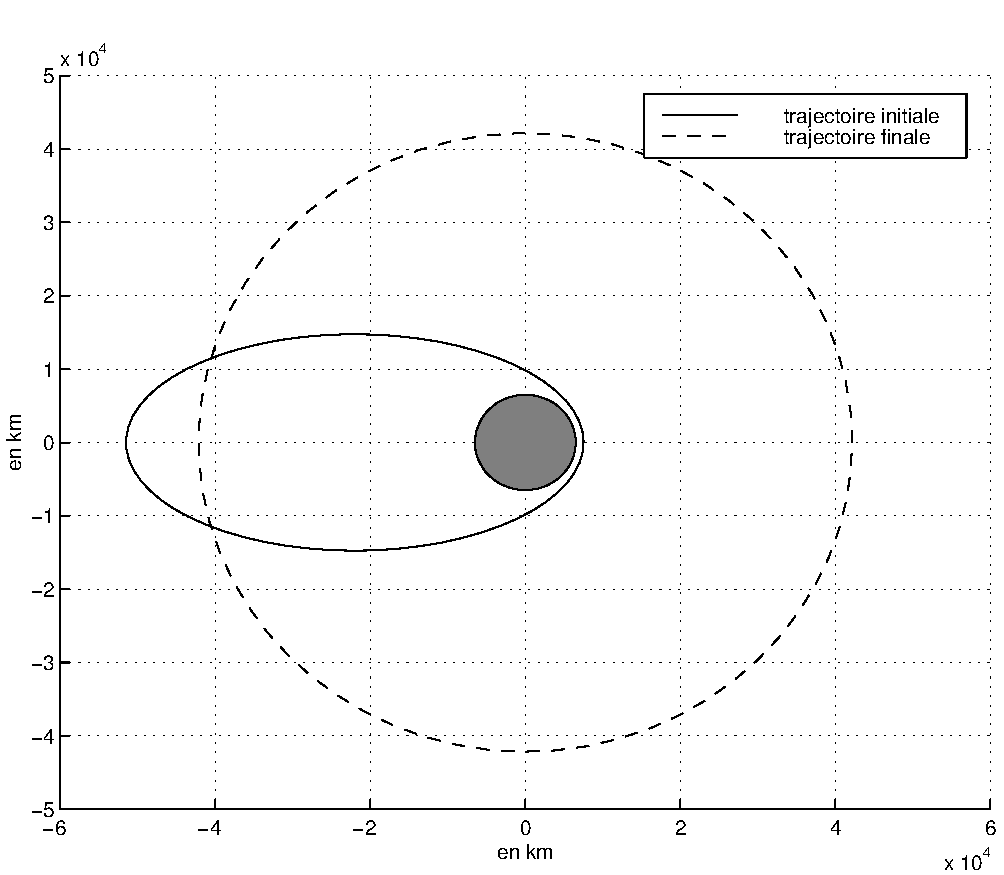
\includegraphics[height=7.0cm,width=8.0cm]{./fig1transfert}
\caption{\label{figtransfert}Transfert orbital 2D.}
\end{figure}

\section{Probl\`eme en temps minimal}

Consid\'erons le probl\`eme de transfert orbital \`a temps minimal suivant~:
\leqnomode
\begin{equation}\label{eq:transfert_temps_min}
    \tagProblem
        \left\{
            \begin{array}{l}
                \displaystyle J(t_f,u(\cdot)) = t_f \longrightarrow \min                                \\[1.0em]
                \displaystyle \dot{x}_1(t) = x_3(t), \\[0.5em]
                \displaystyle \dot{x}_2(t) = x_4(t), \\[0.5em]
                \displaystyle \dot{x}_3(t) = -\frac{\mu\, x_1(t)}{{r(t)}^3} + u_1(t), \\[0.5em]
                \displaystyle \dot{x}_4(t) = -\frac{\mu\, x_2(t)}{{r(t)}^3} + u_2(t),
                \quad \norme{u(t)} \le \gamma_\mathrm{max}, 
                \quad t \in \intervalleff{0}{t_f} \text{ p.p.}, \quad u(t) \coloneqq(u_1(t),u_2(t)),     \\[1.0em]
                \displaystyle x_1(0) = x_{0,1},   \quad x_2(0) = x_{0,2},  \quad x_3(0) = x_{0,3}, \quad x_4(0) = x_{0,4},  \\[1.0em]
                \displaystyle r(t_f)^2 = r_f^2, \quad
                \displaystyle x_3(t_f) = - \sqrt{\frac{\mu}{r_f^3}}\, x_2(t_f), \quad
                \displaystyle x_4(t_f) = \sqrt{\frac{\mu}{r_f^3}}\, x_1(t_f),
            \end{array} 
        \right.
\end{equation}
\reqnomode
avec $r(t) \coloneqq \sqrt{x_1(t)^2 + x_2(t)^2}$. Les unit\'es choisies sont le kilom\`etre pour les distances et l'heure pour les temps, \cf
table \ref{table:transfert_temps_min_data}.

\begin{table}[ht!]
    \centering
    \begin{tabular}{lll}
        \medhrule
        Param\`etre                                & Valeur & Unit\'e   \\
        \bighrule
        $\mu$                   & $5.1658620912\times10^{12}$  & km$^3$ h$^{-2}$ \\
        $r_f$                   & $42165$                           & km \\
        $\gamma_\mathrm{max}$   & $388.8$                           & km h$^{-2}$ \\
        \medhrule
        \\
    \end{tabular}
    \caption{Unit\'e et valeurs des param\`etres constants. Cette valeur de $\gamma_\mathrm{max}$ correspond \`a une acc\'el\'eration de 60N et \`a
    une masse de 2000kg, \cf $\gamma_\mathrm{max} = \frac{F_\mathrm{max}}{m} = \frac{60 \times 3600^2}{2000 \times 10^3} = 388.8$.}
    \label{table:transfert_temps_min_data}
\end{table}

\begin{myQuestion}
    \label{question:transfert_hamiltonien}
    Donner le pseudo-hamiltonien associ\'e au probl\`eme \eqref{eq:transfert_temps_min} (on se placera pour la suite dans le cas normal, \ie $p^0=-1$).
\end{myQuestion}

\begin{myQuestion}
    \label{question:transfert_control}
    Donner le contr\^ole optimal, \ie la loi de commande maximisant le pseudo-hamiltonien.
\end{myQuestion}

\begin{myQuestion}
    \label{question:transfert_fonction_de_tir}
    D\'eterminer la fonction de tir associ\'e \`a \eqref{eq:transfert_temps_min}.
\end{myQuestion}

\begin{myremark}
    Pour la r\'esolution num\'erique, il sera pr\'ef\'erable de remplacer l'\'equation $r(t_f)^2 = r_f^2$ par $r(t_f) = r_f$.
\end{myremark}

\begin{myExercice} Calcul d'une BC-extr\'emale pour le probl\`eme \eqref{eq:transfert_temps_min} avec \hampath.
    \begin{enumerate}
        \item R\'ecup\'erer les sources du sujet 6. Vous pourrez utiliser le script \cmd{orbite0f.m} pour l'affichage des trajectoires.
        \item R\'esoudre la fonction de tir pour les conditions initiales~:
            \[
                x_{0,1} = -44000, \quad x_{0,2} = 0, \quad x_{0,3} = 0, \quad x_{0,4} = -10279.
            \]
            On note $y=(p_0,t_f)$ l'inconnue de la fonction de tir. On prendra comme point de d\'epart pour la commande \cmd{ssolve}
            $y^{(0)} = (10^{-3}, 4\times 10^{-4}, 10^{-3}, 10^{-4}, 4)$.
    \end{enumerate}
\end{myExercice}


